% Pacotes
\usepackage{lipsum}
\usepackage{caption}
\usepackage{graphicx}
    \DeclareCaptionFormat{sanslabel}{#3}%
\usepackage{color}
\usepackage[table]{xcolor}
\usepackage{tikz}
\usepackage{tcolorbox}
\usepackage{amsmath}
\usepackage{amsfonts}
\usepackage{amssymb}
\usepackage{mathrsfs}
\usepackage{mathtools}
\usepackage{enumitem} 
\usepackage{float}
\usepackage[utf8]{inputenc}	
\usepackage[french]{babel}
\usepackage[T1]{fontenc}
\usepackage{caption}
\usepackage{subcaption}
\usepackage{media9}


% Theme choice:
\usetheme{CambridgeUS}

% Cores personalizadas
\definecolor{PROFMATgreen}{RGB}{0, 138, 163}
\definecolor{UFTgreen}{RGB}{0, 137, 124}
\definecolor{UFTblue}{RGB}{0, 84, 132}
\definecolor{UFTyellow}{RGB}{253, 185, 46}
\definecolor{UFTgray}{RGB}{132, 134, 136}

% Ativar numeração de tabelas
\setbeamertemplate{caption}[numbered]

% Definir novo estilo de item com quadrado verde
\setlist[itemize,1]{label=\textcolor{UFTgreen}{\rule{1ex}{1ex}}}

\setbeamercolor*{structure}{bg=UFTgreen,fg=black}

\setbeamercolor*{palette primary}{fg=black,bg=PROFMATgreen}
\setbeamercolor*{palette secondary}{fg=white,bg=UFTblue}
\setbeamercolor*{palette tertiary}{fg=black,bg=UFTgreen}
\setbeamercolor*{palette quaternary}{fg=white,bg=black}

\setbeamercolor{section in toc}{fg=black,bg=white}
\setbeamercolor{alerted text}{fg=white}

\setbeamercolor*{item}{fg=PROFMATgreen}

\setbeamercolor{block title}{bg=UFTgreen,fg=white}
\setbeamercolor{block body}{bg=UFTgray!10,fg=black}

\setbeamercolor{titlelike}{fg=white, bg=UFTblue}
\setbeamercolor{frametitle}{bg=UFTgray!20,fg=UFTgreen}


\setbeamertemplate{title page}{
    \vfill
    \vskip1em\par
    \begingroup
        \centering
        \begin{beamercolorbox}[sep=8pt,center,shadow=true,rounded=false]{title}
            \usebeamerfont{title}\inserttitle\par%
            \ifx\insertsubtitle\@empty%
            \else%
                \vskip0.25em%
                {\usebeamerfont{subtitle}\usebeamercolor[fg]{subtitle}\insertsubtitle\par}%
            \fi%
        \end{beamercolorbox}%
        \vskip0.5em\par
        \begin{minipage}{0.6\linewidth}
            \centering
            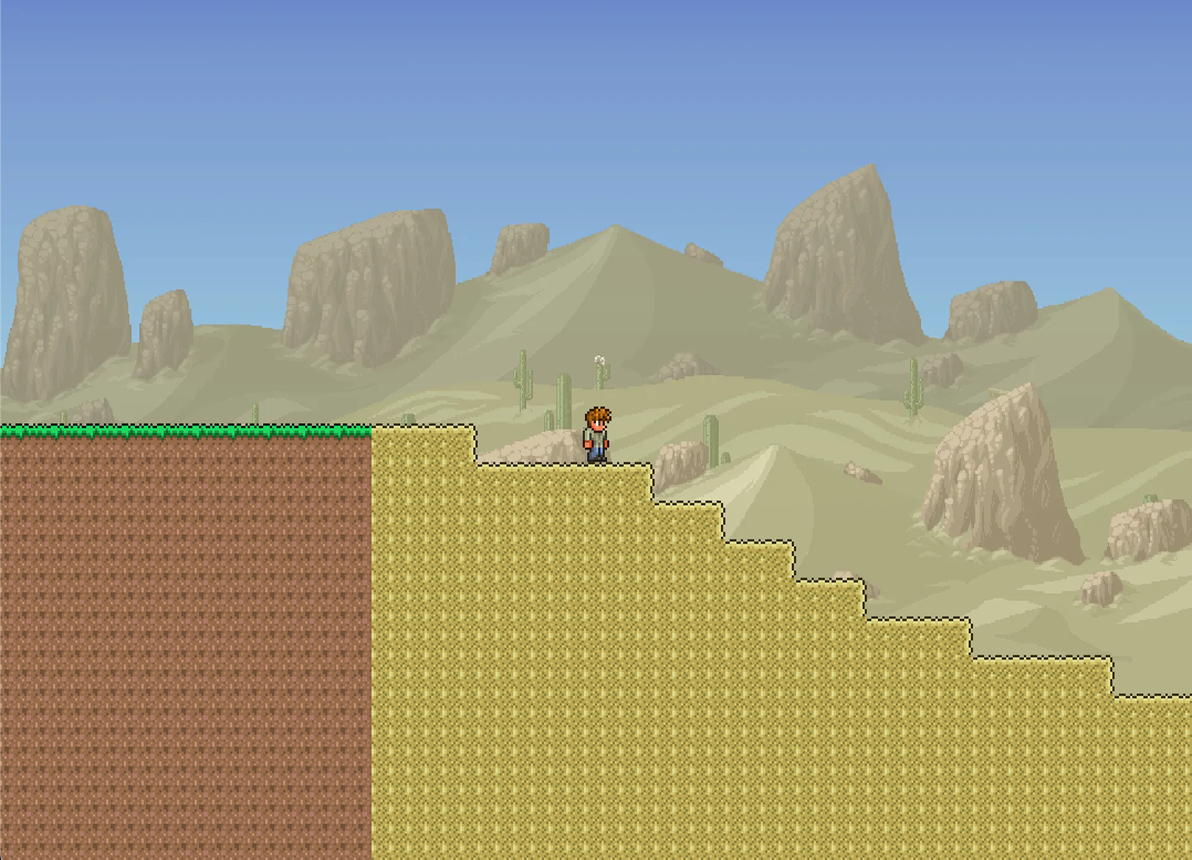
\includegraphics[width=0.6\linewidth]{assets/background_1.png}
        \end{minipage}
        \begin{beamercolorbox}[sep=6pt,center]{author}
            \usebeamerfont{author}\insertauthor
        \end{beamercolorbox}
        \begin{beamercolorbox}[sep=5pt,center]{advisor}
            \usebeamerfont{institute} \advisorname
        \end{beamercolorbox}
        \begin{beamercolorbox}[sep=5pt,center]{institute}
            \usebeamerfont{institute}\insertinstitute
        \end{beamercolorbox}
        \par
    \endgroup
    \vfill
}


% Remover bordas arredondadas dos blocks
\makeatletter
\setbeamertemplate{blocks}[default] % Isso remove o arredondamento
\makeatother


% Pacotes de citações
% ---

\usepackage[alf,abnt-etal-text=it,abnt-repeated-author-omit=yes,abnt-etal-list=0,abnt-etal-cite=3,abnt-emphasize=bf]{abntex2cite}	% Citações padrão ABNT



\setbeamercolor{bibliography entry author}{fg=black}
\setbeamertemplate{bibliography item}{\newblock}


\setbeamertemplate{frametitle continuation}{}

% Redefinir o separador para um traço
% Redefinir o separador
\captionsetup[figure]{labelformat=simple, labelsep=endash, textformat=period, font=footnotesize}


% Redefine espaçamento antes e depois da legenda em figuras e tabelas
\captionsetup[figure]{aboveskip=2pt, belowskip=0pt}


% Define uma penalidade alta para a hifenização
\hyphenpenalty=10000
\tolerance=10000


% Personalizando o estilo da tabela de conteúdos
\setbeamertemplate{section in toc}[sections numbered]
\renewcommand{\thesection}{\textcolor{PROFMATgreen}{\arabic{section}}}
\renewcommand{\thesubsection}{\textcolor{PROFMATgreen}{\arabic{section}.\arabic{subsection}}}

\setbeamersize{text margin left=0.8cm, text margin right=0.8cm}

